\documentclass[12pt]{report}
\usepackage[utf8]{inputenc}
\usepackage{graphicx}
\usepackage{subcaption}
\usepackage{setspace}
\usepackage[english]{babel}
\usepackage{wrapfig}
\usepackage[font=small,labelfont=bf]{caption}

\doublespacing

\graphicspath{{Images/}}
\title{Thesis}
\author{John DeCorato}
\date{ }

\setlength{\parindent}{3em}
\setlength{\parskip}{1em}

\begin{document}

\chapter{Line Rendering}

Drawing lines on a computer is an easy problem to solve. 
However, drawing lines well is significantly more difficult.
While OpenGL is known for it's GPU rendering capabilities with many different types of triangle primitives, it's line rendering capabilities are rather weak.
The GL\_LINES drawing mode does not support line joins, line caps, non-integer line widths, widths greater than 10px, or varying widths in a single pass.
Because of these limitations, it is unsuitable for line rendering for high quality sketching applications.
Additionally, OpenGL's line anti-aliasing is both inconsistant in it's device support and poor in quality.

We would like to have a wide variety of line styles for the user to draw with, for example.
The common approach for making production quality lines is to transform the lines into triangles. 
Using triangles gives a much higher level of control over how the line is drawn because we are not bound to the original definition of the line.

\begin{figure}
\includegraphics[width=\linewidth]{opengllines}
\caption{An example of native line rendering in OpenGL using GL\_LINES. Notice the poor anti-aliasing and holes from no joins.}
\end{figure}

\section{Creating Geometry From the Line Definition}


Starting the line is straight forward. 
Assuming we are given a set of points and a line width, we can start drawing the line by creating a line segment between a set of two points. We then extrude the segment along the positive and negative normal by half of the line width.
However, a problem arises when multiple of these segments are formed along the line points.
We begin to get gaps along the drawn line. 
To solve this, we need to create a join between each of the line segments.
There are three main join types commonly used to solve this problem: miter, bevel, and round joins.

\begin{figure}
	\includegraphics[width=\textwidth]{linesegment1.png}
	\caption{Diagram for creating the line geometry}
\end{figure}

\begin{figure}
	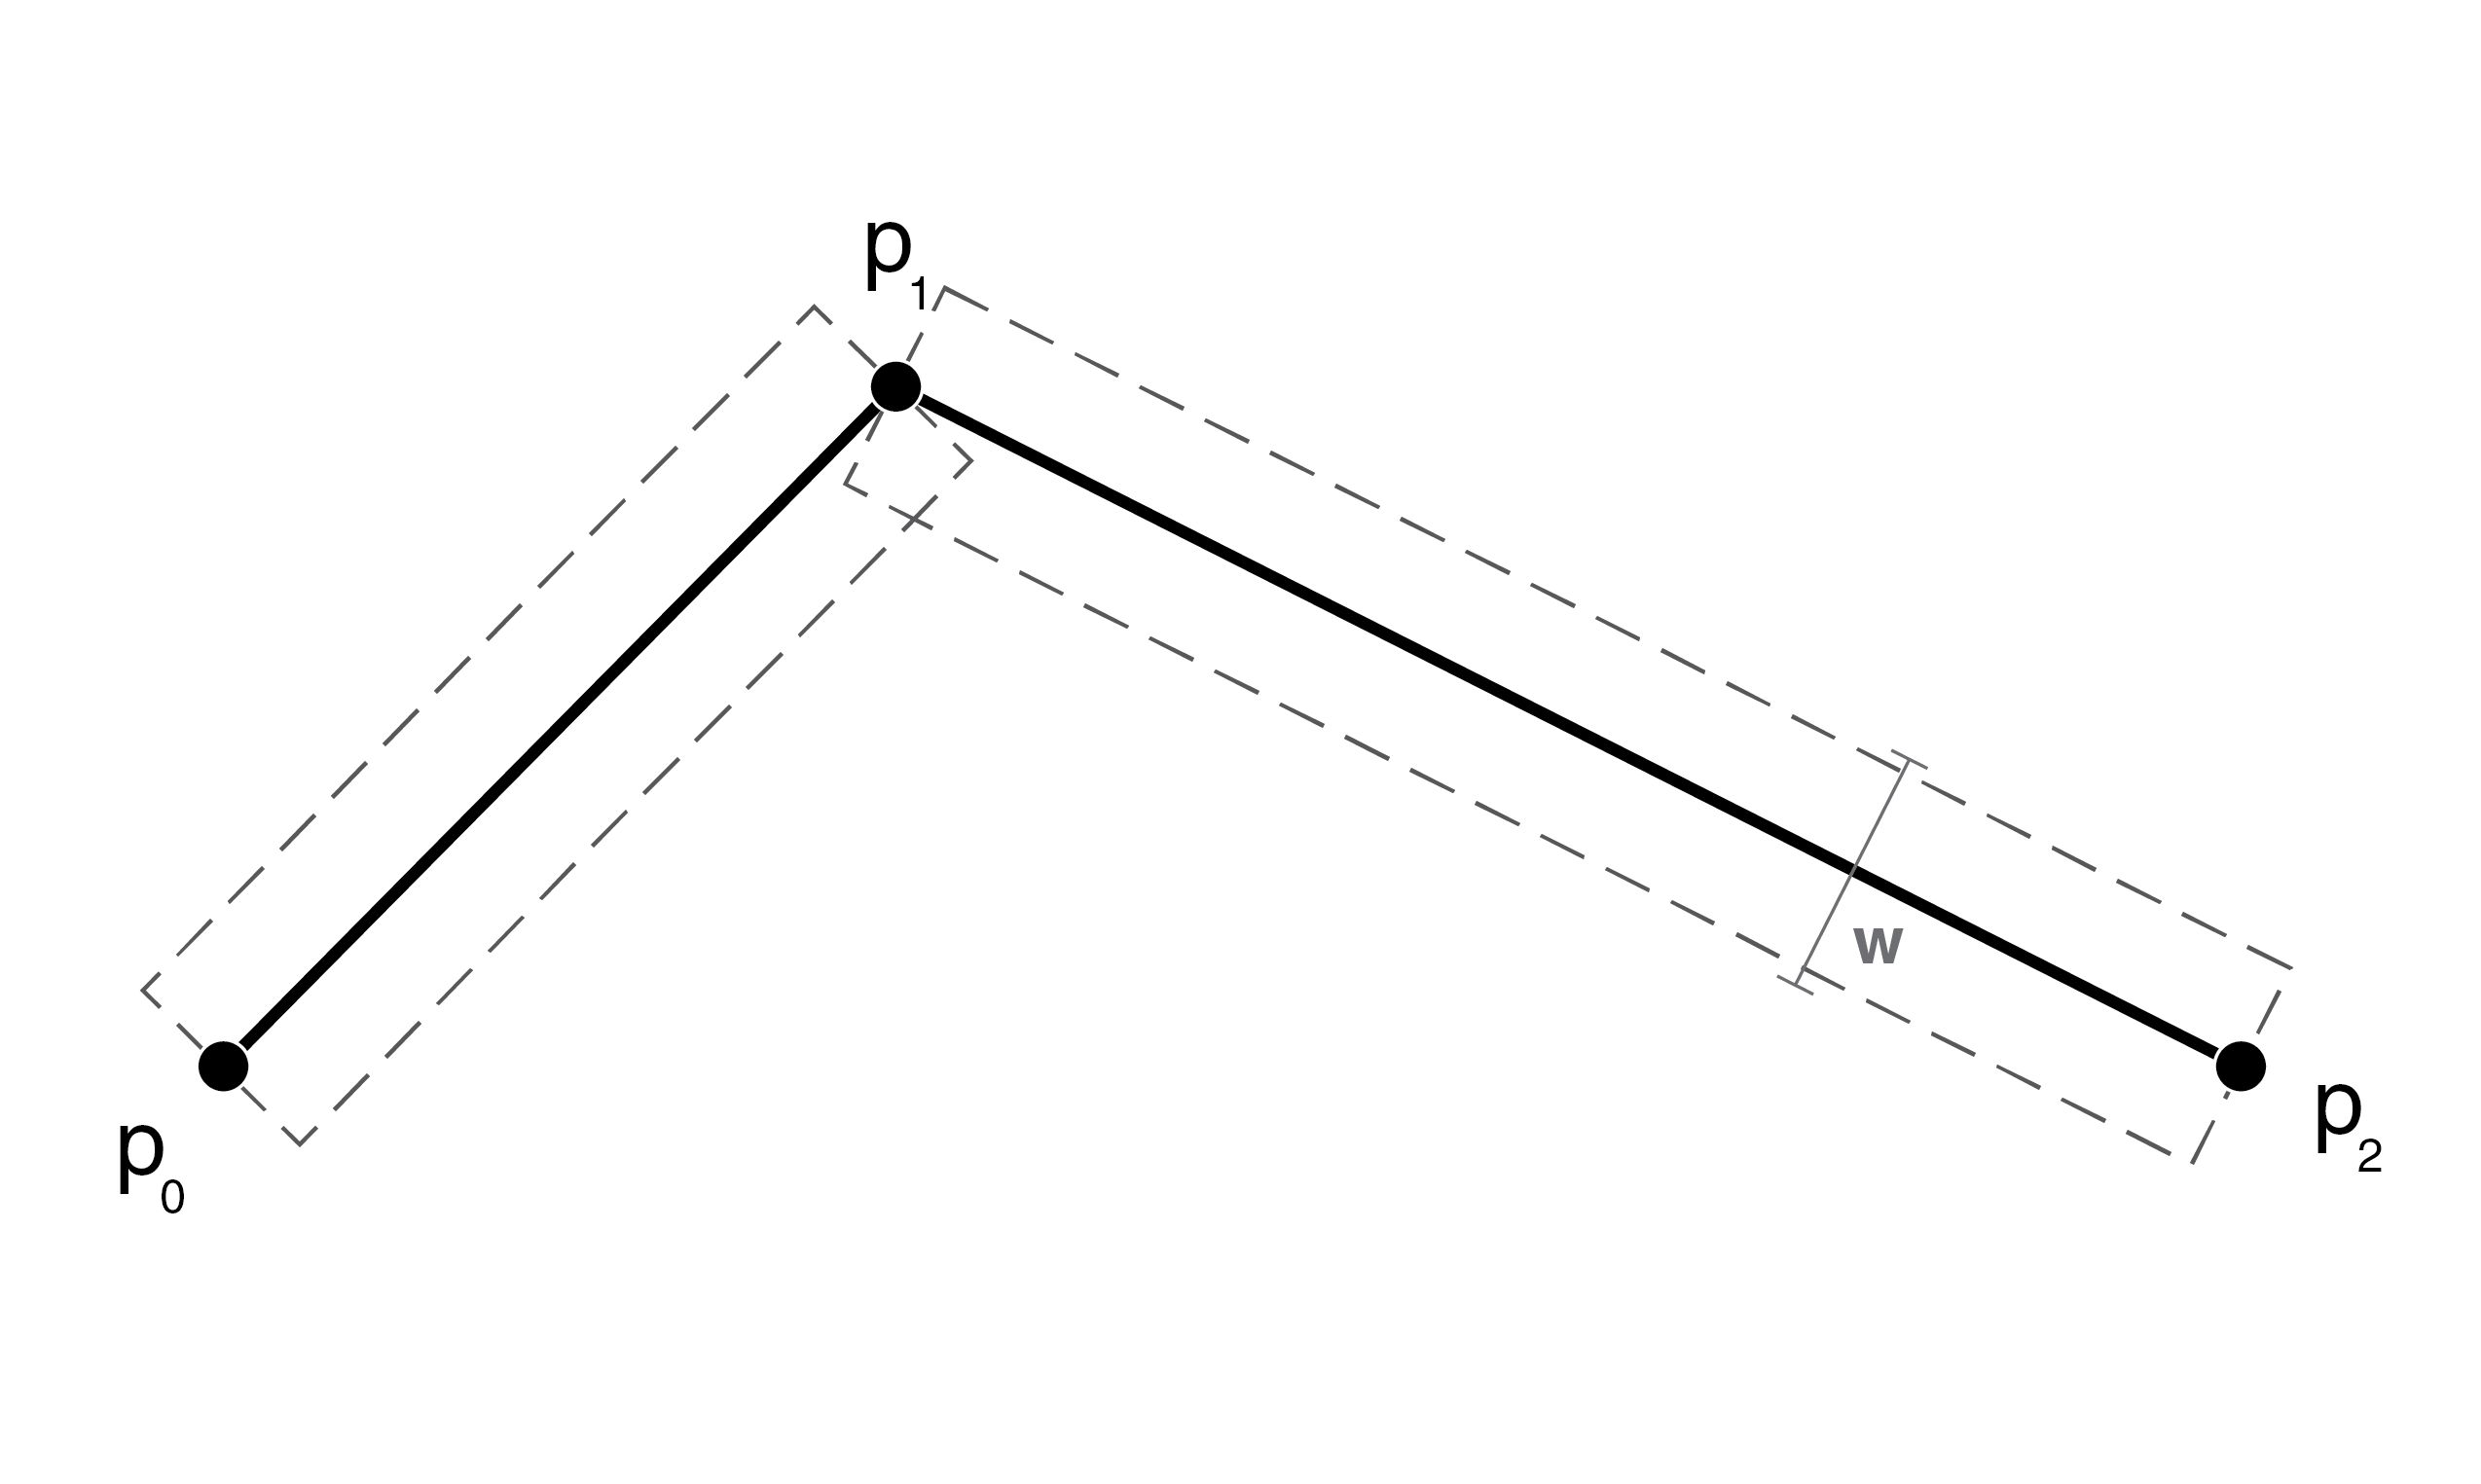
\includegraphics[width=\textwidth]{linesegment2.png}
	\caption{The gap that forms when connecting segments}
\end{figure}

\begin{figure}
	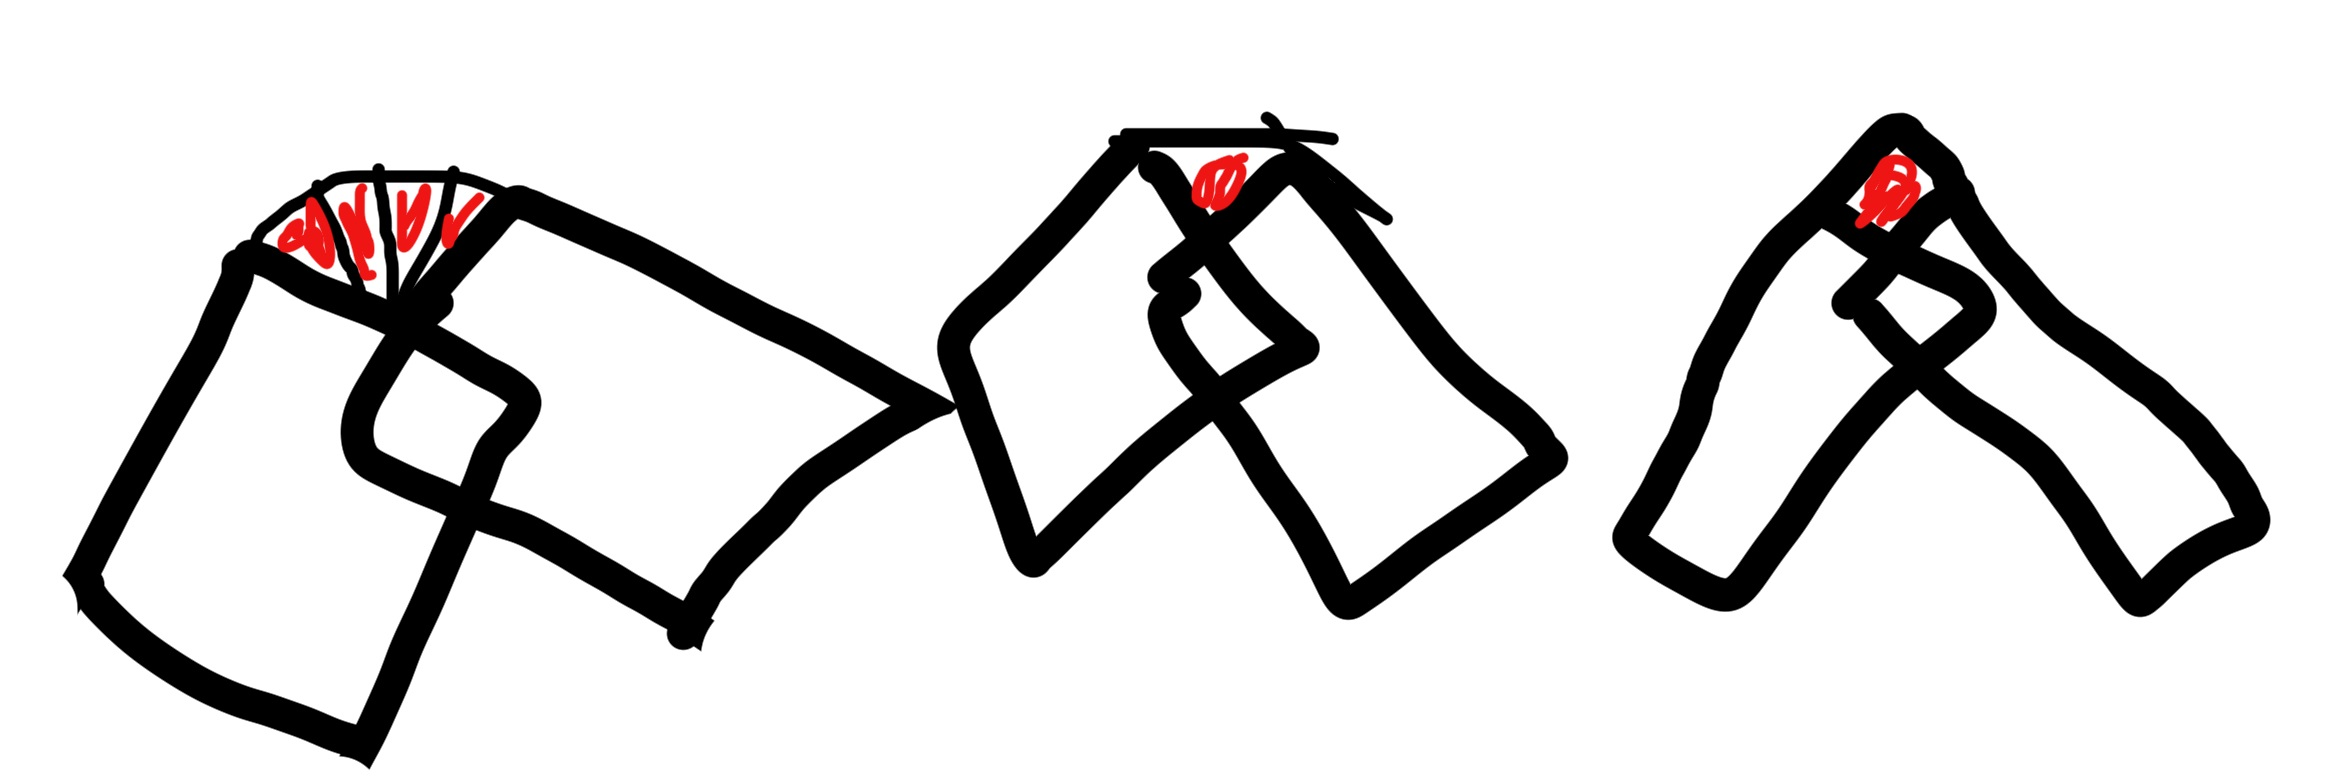
\includegraphics[width=\textwidth]{jointypes.jpg}
	\caption{Types of joins from left to right: round, bevel, miter}
\end{figure}
The round join is formed by rounding out the gap such that a smooth curve is created. 
It is calculated by forming a circle whose center is the line point at the gap, with a radius of half of the total line width. 
From there, the part of the circle that fills in the gap is polygonalized.
The bevel join is formed by simply filling in the triangular shaped hole with a polygon. 
The polygon's third edge is the line segment formed from $p_1a$ and $p_1b$ (note change names when adding better diagram with labels).

\noindent \textbf{TODO}: Add derivation and diagrams for miter join.

Miter joins have the particular issue that artifacts can arise from exceptionally sharp points in the line segments. 
This should be avoided with splines since the spline should subdivide in these cases.

\begin{figure}
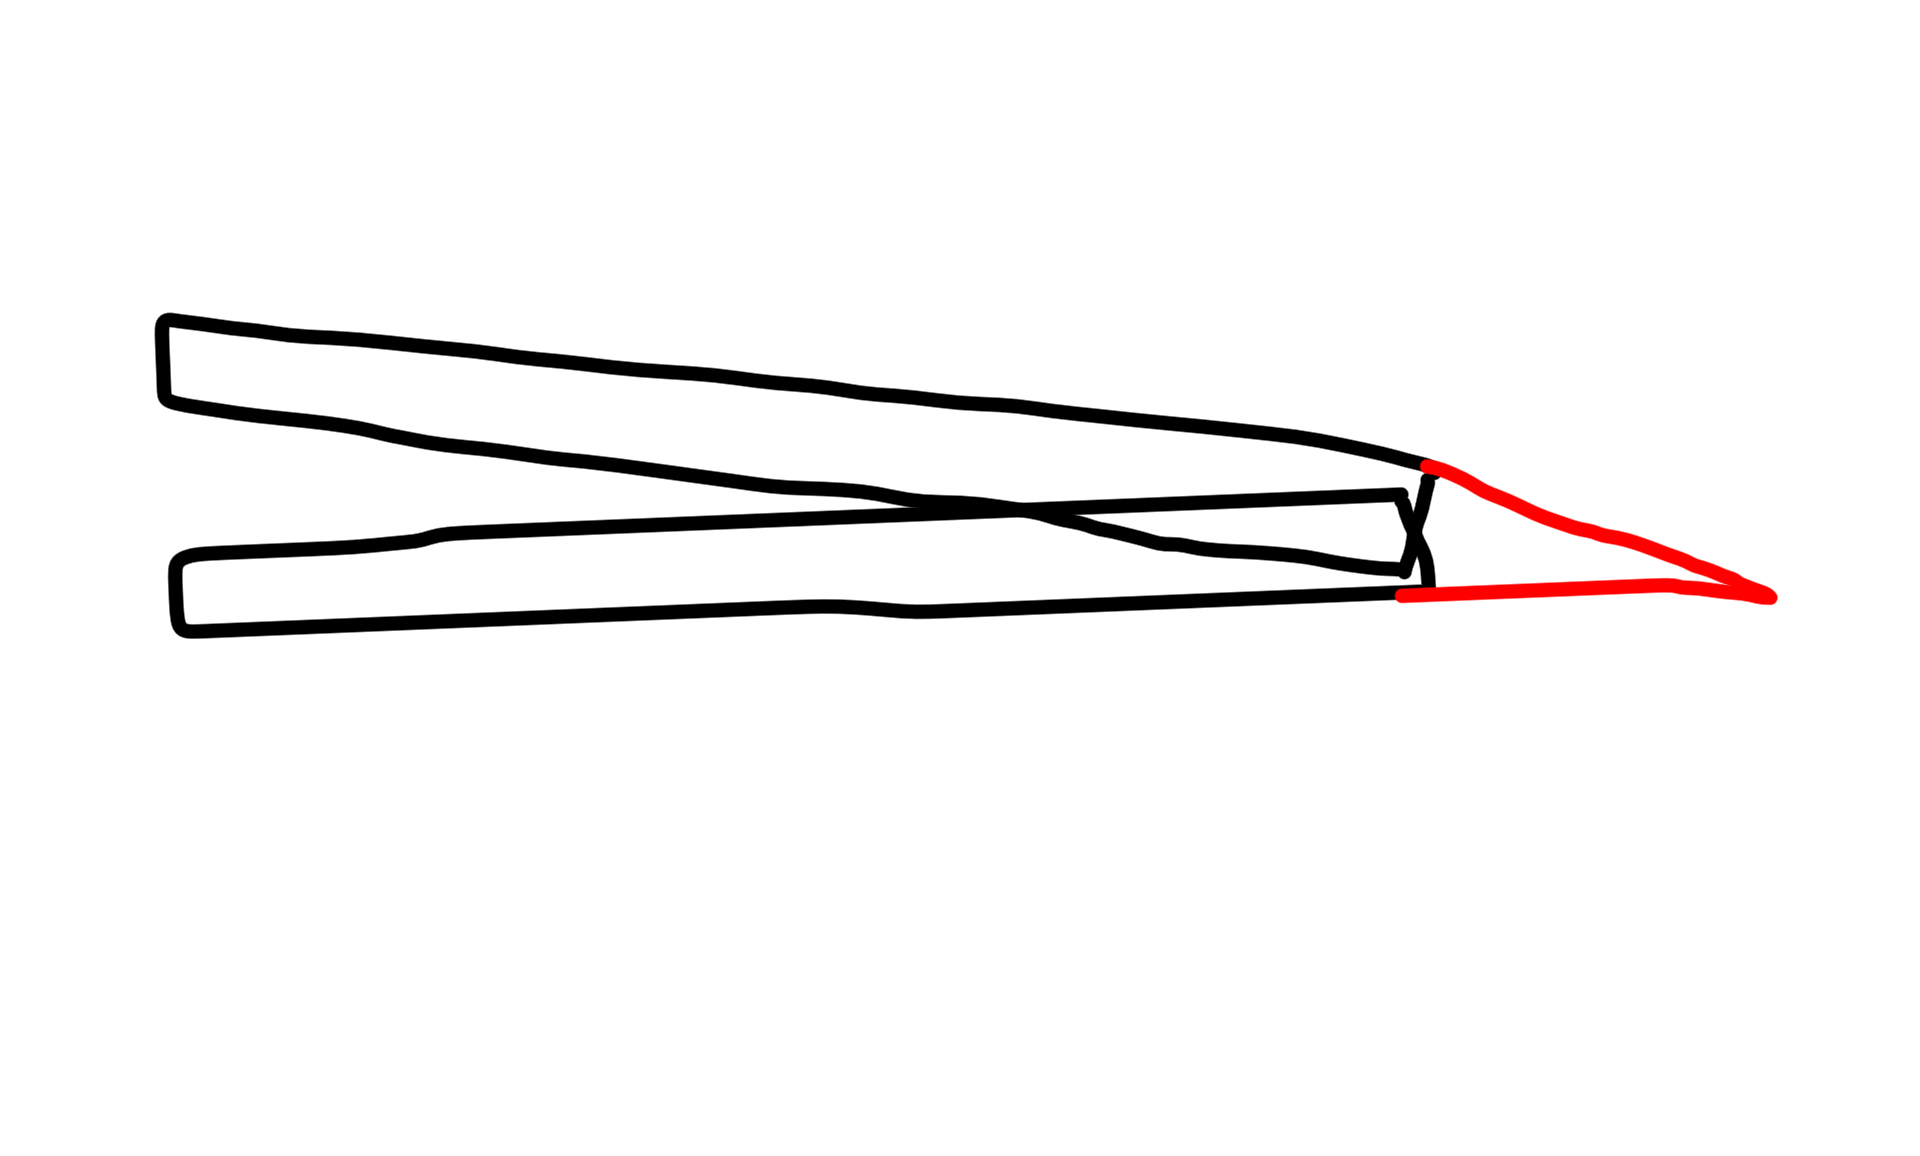
\includegraphics[width=\textwidth]{miterartifact.jpg}
\caption{An example of a miter join artifact from a sharp curve}
\end{figure}

\section{Implementation}

Actually creating this geometry can get very expensive, especially as more and more lines are drawn. 
To make this as cheap as possible we take advantage of the properties of both miter joins and our spline storage.
The miter join has the advantage of being able to be added by simply translating and fusing vertices in the rectangular geometry. 
This allows for the least complexity in forming line geometry by simply creating two vertices for each defined line point, which are used to define a triangle strip. 
Then, using a vertex shader, the vertex positions are transformed appropriately to form the line polygon.

\begin{figure}
	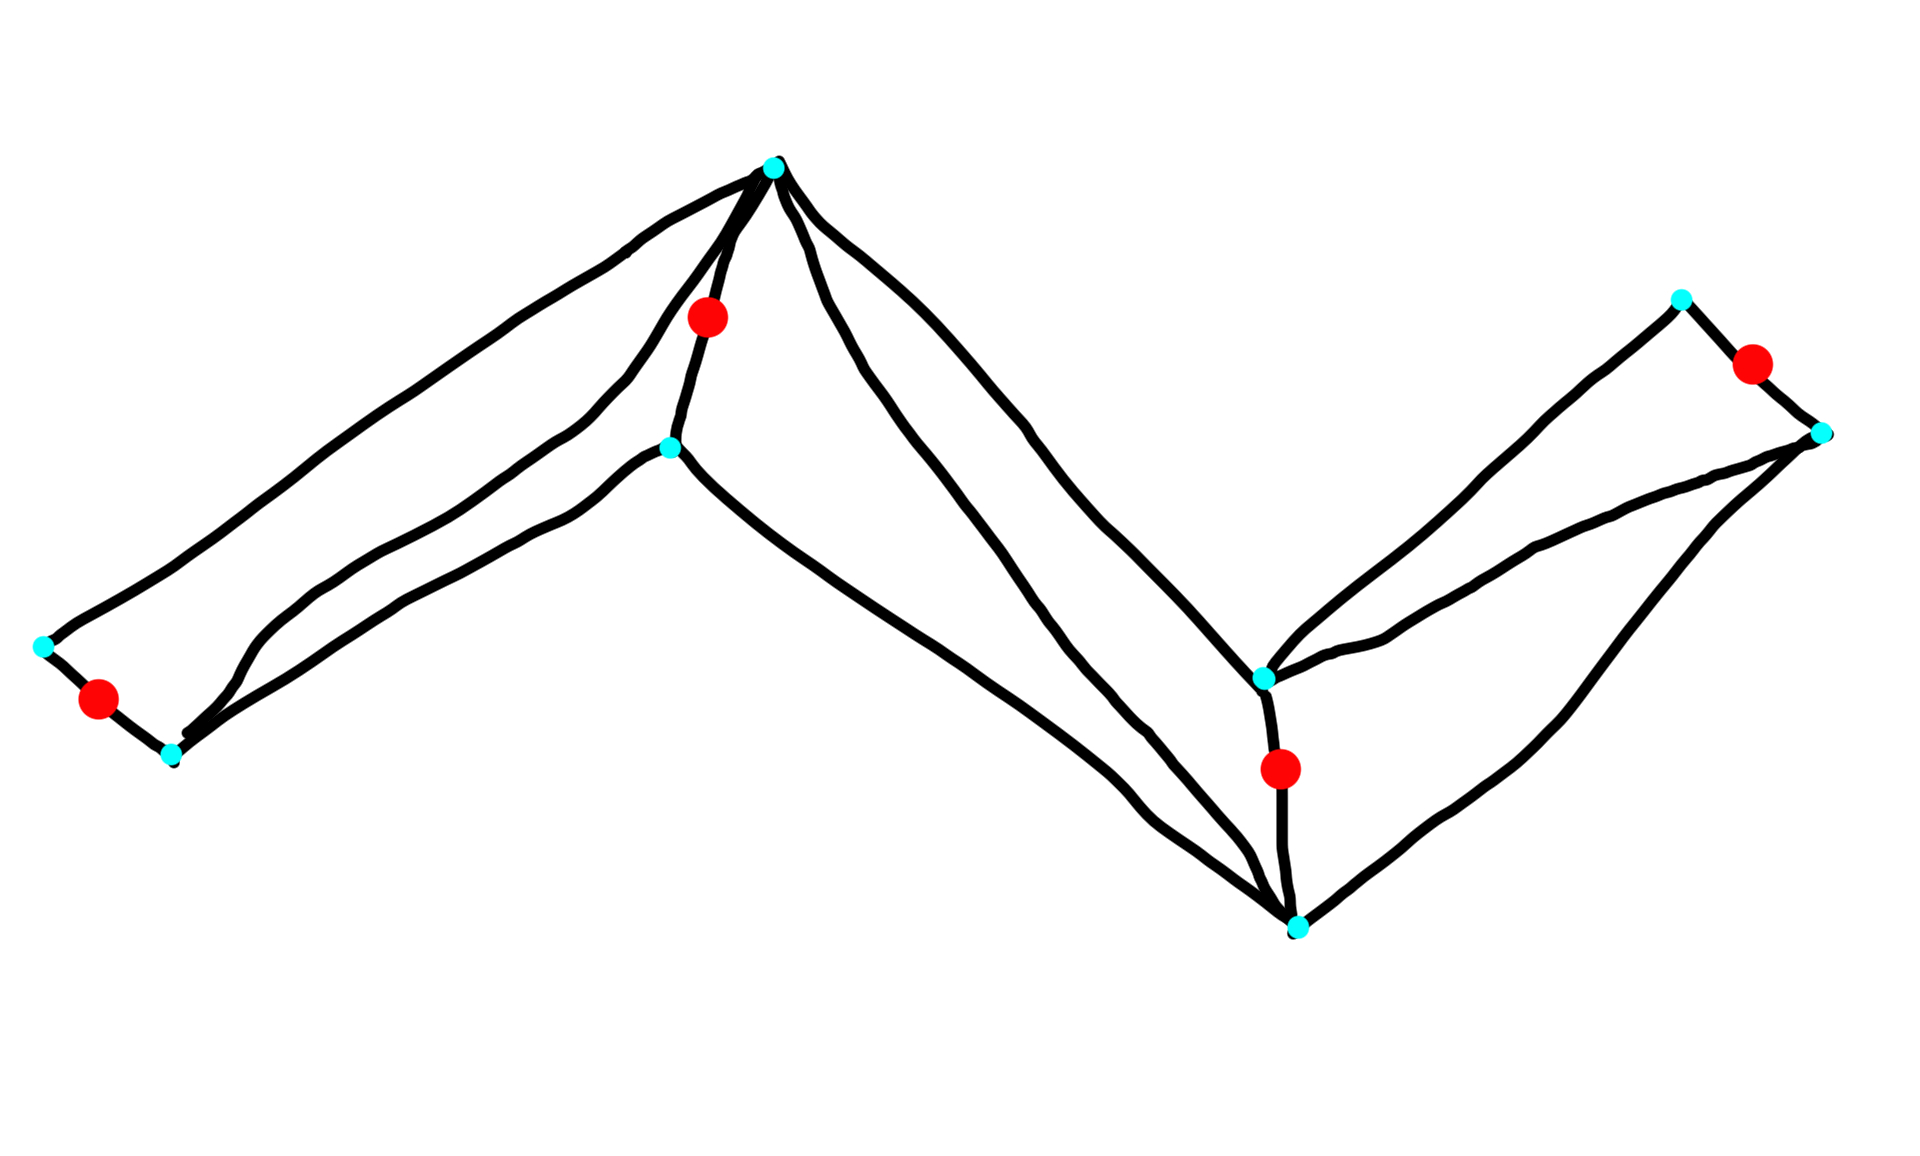
\includegraphics[width=\textwidth]{miterpolys.jpg}
	\caption{Polygonization of a line with miter joins using only two vertices per control point}
\end{figure}

\begin{figure}
	\begin{center}
		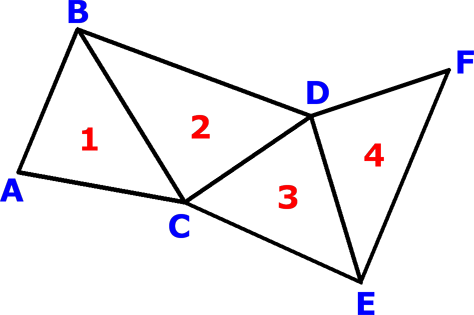
\includegraphics[width=\textwidth]{trianglestrip.png}
	\end{center}
	\caption{A standard triangle strip. Note how the definition matches our polygonalization}
\end{figure}

The system can now display polygonalized, three dimensional lines and does so efficiently.
However, there are two problems with this approach.
First, lines only exist in the plane they are drawn in.
This means if the camera were to rotate such that it is perpendicular to the plane the lines were drawn on, the lines would disappear from our rendering.
This happens because we currently expand the lines in world space, based on the  plane the line was drawn on, instead of based on the current position of the camera.
Second, this approach assumes we expand our lines on a plane, limiting the sketching surfaces available.
Expanding the lines if the sketch was done on a sphere becomes a significantly harder problem. how is line width defined on curved geometry? 
How do we create them without creating too many polygons and running out of memory?
Luckily, we can avoid both of these problems by instead doing a screen space projection of the points that form our lines, and then expand them in the "two-dimensional" screen space.
This means that no matter how the line is drawn in the 3-D environment, their definition doesn't change.

The basic algorithm is:
\begin{enumerate}
\item Begin with three points, the current, previous, and next points along the polyline.
\item Use the Model-View-Projection matrix to project these points into clip space
\item Convert from clip space into normalized device coordinates
\item Compute the normal for each of the line segments
\item Expand along the screen space normal, and compute a join
\end{enumerate}
For the beginning and the ends of the line, we duplicate the second and second-to-last points on the polyline to avoid branching in the vertex shader. 


\end{document}